\documentclass{beamer}

\input{../../spec_files/course_preamble.tex}
\subtitle{Foundations of Neuro-Symbolic AI}
\date{Summer Term 2026}
\author[FONS]{Alex Goessmann}
\institute[]{
    University of Applied Science Würzburg-Schweinfurt
%    Weierstrass Institute for Applied Analysis and Stochastic
}

%\newcommand{\techwstitle}{
%\small
%%Workshop \\
%Logik für Erklärbare KI:
%Technische Einführung in das ENEXA Projekt}
%\newcommand{\smalltechwstitle}{ENEXA Workshop}

%\newcommand{\techwsdate}{15.+16. July, 2024}

%\newcommand{\techwsauthors}{
%Alex Goessmann
%}

%\newcommand{\techwsinclude}{
%	\usepackage{../../spec/beamercolorthemeclaw}
%	\usepackage{/Users/alexgoessmann/Documents/ENEXA/latex_macros/beamer_template/beamerfontthemeclaw}
%	\usepackage{/Users/alexgoessmann/Documents/ENEXA/latex_macros/beamer_template/beamerinnerthemeclaw}
%	\usepackage{/Users/alexgoessmann/Documents/ENEXA/latex_macros/beamer_template/beamerouterthemeclaw}
%
%	\input{/Users/alexgoessmann/Documents/ENEXA/latex_macros/packages.tex}
%	\input{/Users/alexgoessmann/Documents/ENEXA/latex_macros/macros.tex}
%	\input{/Users/alexgoessmann/Documents/ENEXA/latex_macros/macros_tc.tex}
%	\input{/Users/alexgoessmann/Documents/ENEXA/latex_macros/tikz_blocks.tex}
%
%	\subtitle{\techwstitle}
%	\date[\techwsdate]{\techwsdate}
%	\author[\smalltechwstitle]{\techwsauthors}
%	\institute[]{\eupic}
%}

\newcommand{\techwschapterone}{I-Tensors}
\newcommand{\techwschaptertwo}{II-Probabilities}
\newcommand{\techwschapterthree}{III-Logics}
\newcommand{\techwschapterfour}{IV-Applications}

\newcommand{\eupic}{
\begin{center}
	%\includegraphics[width=4cm]{/Users/alexgoessmann/Documents/ENEXA/latex_macros/images/fundedEU.png}
\end{center}
}

\newcommand{\enexadateveublock}{
\begin{center}\begin{tikzpicture}
  	%\node [anchor=center] at (0,0) {\includegraphics[width = 1.5cm]{/Users/alexgoessmann/Documents/ENEXA/latex_macros/images/DATEV.png}};
	%\node [anchor=center] at (2.5,0.5) {\includegraphics[width = 3.5cm]{/Users/alexgoessmann/Documents/ENEXA/latex_macros/images/enexa.png}};
	%\node [anchor=center] at (2.55,-0.5) {\includegraphics[width = 3cm]{/Users/alexgoessmann/Documents/ENEXA/latex_macros/images/fundedEU.png}};
\end{tikzpicture}\end{center}
}


%% OLD
\newcommand{\aselectionvariable}{L}
\newcommand{\vselectionvariable}{L}
\newcommand{\fselectionvariable}{L}
\newcommand{\cselectionvariable}{L}
\newcommand{\individualorder}{n}
\newcommand{\variableof}[1]{\indvariableof{#1}}
\newcommand{\sindex}{s}
\newcommand{\pindex}{p}
\newcommand{\oindex}{o}
\newcommand{\exquery}{q}
%\newcommand{\datapointof}[1]{x^{#1}}
\newcommand{\atomicqueryof}[1]{g_{#1}}
\newcommand{\facsystem}{\shortcatvariables}
\newcommand{\margprobof}[1]{\probat{#1}}
\newcommand{\mlnprobabilityof}[1]{\expdistof{#1}}
%\newcommand{\oldenexadateveublock}{
%	\begin{center}
%	\begin{minipage}{0.2\textwidth}
%		\begin{center}
%			\includegraphics[width = 2.5cm]{images/DATEV.png}
%		\end{center}
%	\end{minipage}
%	\begin{minipage}{0.55\textwidth}
%		\begin{center}
%			\includegraphics[width=5.5cm]{images/enexa.png} \\
%			\includegraphics[width=5.5cm]{images/fundedEU.png} \\
%		\end{center}
%	\end{minipage}
%	\end{center}
%}

\title[Tensor Networks]{
	\techwschapterone \\
	{\huge Formalization of Tensor Networks}
}

\begin{document}

{\frame[plain]{\titlepage}}


\begin{frame}{Tensor Networks}

Tensor Networks are build by
\begin{itemize}
	\item Separated Combination of Tensors $\hypercoreof{\edge_1},\hypercoreof{\edge_2}, \hypercoreof{\edge_3}$: \emph{Tensor Products}
	\only<2->{
	\item Connecting Tensors along common legs and closing legs: \emph{Contractions}
	}
\end{itemize}

\vfill

\begin{center}
	\begin{tikzpicture}[scale=0.35,thick] % , baseline = -3.5pt


\only<1>{\draw (0,-3)--(0,-5) node[midway,right] {\tiny $\catvariableof{0}$}; }
\only<2->{\draw (0,-3)--(0,-4) node[midway,right] {\tiny $\catvariableof{0}$}; }

\only<1->{

\draw (-1,-1) rectangle (5,-3);
\node[anchor=center] (text) at (2,-2) {\small $\hypercoreof{\edge_1}$};


\draw (2,-3)--(2,-5) node[midway,right] {\tiny $\catvariableof{1}$};
\draw (4,-3)--(4,-5) node[midway,right] {\tiny $\catvariableof{2}$};


\draw (6,-1) rectangle (10,-3);
\node[anchor=center] (text) at (8,-2) {\small $\hypercoreof{\edge_3}$};
\draw (7,-3)--(7,-5) node[midway,right] {\tiny $\catvariableof{2}$};
\draw (9,-3)--(9,-5) node[midway,right] {\tiny $\catvariableof{3}$};

\begin{scope}[shift={(0,-2)}]
\draw (1,-7) rectangle (5,-9);
\node[anchor=center] (text) at (3,-8) {\small $\hypercoreof{\edge_2}$};
\draw (2,-5)--(2,-7) node[midway,right] {\tiny $\catvariableof{1}$};
\draw (4,-5)--(4,-7) node[midway,right] {\tiny $\catvariableof{2}$};

\end{scope}
}

\only<2->{
\draw (2,-5)--(2,-7);

\draw (4,-5) to[bend right=20]  (7,-6); % node[midway,left] {\tiny $\catvariableof{2}$};
\draw (4,-7) to[bend right=-20]  (7,-6); 

\draw[fill] (2,-6) circle (0.25cm);
\draw (2,-6) to[bend right=20] (-1,-8); % node[midway, right]{\tiny $\catvariableof{1}$};
\node[anchor=center] (text) at (-2,-8) {\tiny $\catvariableof{1}$};

\draw[fill] (7,-6) circle (0.25cm);
\draw (7,-5) -- (7,-6);
\draw (7,-6)--(7,-7) node[midway,right] {\tiny $\catvariableof{2}$};


\draw (-1,-4) rectangle (1,-6);
\node[anchor=center] (text) at (0,-5) {\small $\ones$};
\draw (6,-7) rectangle (8,-9);
\node[anchor=center] (text) at (7,-8) {\small $\ones$};
}



\end{tikzpicture}
\end{center}


\end{frame}


\section{Tensor Products}

\begin{frame}{Separated Combination of Tensors: \\ Tensor Products}

\begin{definition}[Tensor Product]\label{def:tensorProduct}
	Let there be two tensor
	\begin{align*}
		\hypercore \facstates \rightarrow \rr \quad \text{and} \quad  \sechypercore \facstates \rightarrow \rr \, . 
	\end{align*}
	Then there tensor product is the map
	\begin{align*}
		\hypercore \otimes \sechypercore :  \left(\facstates\right) \times \left(\secfacstates\right) \rightarrow \rr
	\end{align*}
	defined for $\catindices\in\facstates$ and $\seccatindices\in\secfacstates$ as
	\begin{align*}
		\hypercore \otimes \sechypercore(\catindices,\seccatindices) 
		=  \hypercore(\catindices)\cdot \sechypercore(\seccatindices) \, .
	\end{align*}
\end{definition}

\end{frame}




\begin{frame}{Example}

\textbf{Example:} The one-hot encoding $\onehotmapof{(0,2,1)} \in  \bigotimes_{\atomenumerator\in[3]}\rr^4$
	with the coordinates 
\begin{align*}
	\onehotmapof{(0,2,1)}(\catindexof{0},\catindexof{1},\catindexof{2}) = \begin{cases}
	1 & \text{  if  } \catindexof{0} = 0, \,\, \catindexof{1} = 2 \text{  and  } \catindexof{2} = 1 \\
	0 & \text{ else}
	\end{cases}
\end{align*}
is the tensor product of 
\begin{align*}
	\onehotmapof{(0)}(\catindexof{0}) = \begin{cases}
	1 & \text{  if  } \catindexof{0} = 0 \\
	0 & \text{ else}
	\end{cases} 
	\quad  , \quad 
	\onehotmapof{(2)}(\catindexof{1}) = \begin{cases}
	1 & \text{  if  } \catindexof{1} = 2 \\
	0 & \text{ else}
	\end{cases} 	
\end{align*}
and
\begin{align*}
	\onehotmapof{(1)}(\catindexof{2}) = \begin{cases}
	1 & \text{  if  } \catindexof{2} = 1 \\
	0 & \text{ else}
	\end{cases} \, .
\end{align*}


\end{frame}


\begin{frame}{Generic one-hot encodings}
	\begin{definition}[One-hot encoding of Factored Systems]
		The one-hot encoding of a factored systems with variables $\{\catvariableof{\atomenumerator} \, : \, \atomenumeratorin \}$ in state $\catindices$ is the tensor product 
 		\begin{align}
			\onehotmapof{(\catindices)} = \bigotimes_{\atomenumeratorin} \onehotmapof{\catindexof{\atomenumerator}} 
		\end{align}
		of the one-hot encodings of the variables.
	\end{definition}
	We can depict the one-hot encoding by
	\begin{center}
		\begin{tikzpicture}[scale=0.35,thick] % , baseline = -3.5pt


\draw (-12,1) rectangle (-3,3);
\node[anchor=center] (text) at (-7.5,2) {\corelabelsize $\bigotimes_{\atomenumeratorin} \onehotmapof{\catindexof{\atomenumerator}}$};
\draw (-11,1)--(-11,-1) node[midway,right] {\colorlabelsize $\catvariableof{0}$};
\draw (-9.5,1)--(-9.5,-1) node[midway,right] {\colorlabelsize $\catvariableof{1}$};
\node[anchor=center] (text) at (-6.75,0) {$\cdots$};
\draw (-4,1)--(-4,-1) node[midway,right] {\colorlabelsize $\catvariableof{\atomorder\shortminus1}$};


\node[anchor=center] (text) at (-1,2) {\corelabelsize ${=}$};

\draw (1,1) rectangle (3,3);
\node[anchor=center] (text) at (2,2) {\corelabelsize $\onehotmapof{\catindexof{0}}$};
\draw (2,1)--(2,-1) node[midway,right] {\colorlabelsize $\catvariableof{0}$};

\node[anchor=center] (text) at (4.5,2) {$\otimes$};

\draw (6,1) rectangle (8,3);
\node[anchor=center] (text) at (7,2) {\corelabelsize $\onehotmapof{\catindexof{1}}$};
\draw (7,1)--(7,-1) node[midway,right] {\colorlabelsize $\catvariableof{1}$};

\node[anchor=center] (text) at (9.5,2) {$\otimes$};

\node[anchor=center] (text) at (11,2) {$\cdots$};

\node[anchor=center] (text) at (12.5,2) {$\otimes$};


\draw (14,1) rectangle (16,3);
\node[anchor=center] (text) at (15,2) {\corelabelsize $\onehotmapof{\catindexof{\atomorder\shortminus1}}$};
\draw (15,1)--(15,-1) node[midway,right] {\colorlabelsize $\catvariableof{\atomorder\shortminus1}$};





\end{tikzpicture}
	\end{center}
\end{frame}




%\begin{frame}{Curse of dimensionality of factored representations}
%
%One-hot encodings of the state of factored systems are elements of the tensor space
%	\[ \bigotimes_{\atomenumeratorin} \rr^{\catdimof{\atomenumerator}} \]
%with dimension 
%	\[ \mathrm{dim}\left[ 
%	\bigotimes_{\atomenumeratorin} \rr^{\catdimof{\atomenumerator}} 
%	\right] =
%	\prod_{\atomenumeratorin}  \catdimof{\atomenumerator} \, . \]
%
%Even if we have found a way to depict these objects without specifying all coordinates:
%	\begin{center}
%		How can we apply the tensor formalism to overcome the curse of dimensionality?
%	\end{center}
%
%\end{frame}





\section{Contractions: Decorated Hypergraphs}



\begin{frame}{Depicting common legs: Hypergraphs}

\begin{definition}{Hypergraph}
	A hypergraph $\graph=(\nodes,\edges)$ consists of two sets:
	\begin{itemize}
		\item Nodes $\node\in\nodes$ 
		\item Hyperedges $\edge\in\edges$, where each is is a subset $\edge\subset\nodes$ of nodes
	\end{itemize}
\end{definition}


We depict nodes by gray circles and hyperedges as connections of them:
\begin{center}
	\begin{tikzpicture}[scale=0.35,thick] % , baseline = -3.5pt



\node [circle, draw, thick, fill=gray!50, minimum size = \nodeminsize] (P1) at (0,-3) {\tiny $0$};	
\node [circle, draw, thick, fill=gray!50, minimum size = \nodeminsize] (P2) at (3,-3) {\tiny $1$};
\node [circle, draw, thick, fill=gray!50, minimum size = \nodeminsize] (P3) at (6,-3) {\tiny $2$};

\node [circle, draw, thick, fill=gray!50, minimum size = \nodeminsize] (P4) at (9,-3) {\tiny $3$};;


\draw (P1) to[bend right=-20] (3,0);
\draw (P2) to[bend right=0] (3,0);
\draw (P3) to[bend right=20] (3,0);
\node[anchor=center] (text) at (3,0.5) {$\edge_1 = \{0,1,2\}$};

\draw (P2) to[bend right=20] (4.5,-6);
\draw (P3) to[bend right=-20] (4.5,-6);

\node[anchor=center] (text) at (3,-6.5) {$\edge_2 = \{1,2\}$};

\draw (P3) to[bend right=20] (7.5,-6);
\draw (P4) to[bend right=-20] (7.5,-6);

\node[anchor=center] (text) at (9,-6.5) {$\edge_3 = \{2,3\}$};





\end{tikzpicture}
\end{center}
In this example:
\begin{itemize}
	\item $\nodes = \{0,1,2,3\}$
	\item $\edges = \big\{ \{0,1,2\}, \{1,2\}, \{2,3\}  \big\}$
\end{itemize}

\end{frame}


\begin{frame}{Associating tensors with hyperedges}

Let us use the hypergraph formalism to depict tensor networks
\begin{itemize}
	\item Nodes are decorated by the categorical variables on the tensor legs:
		\[  \{0,\ldots,\atomorder-1\} \quad \text{represent the variables } \quad \{\catvariableof{0},\ldots,\catvariableof{\atomorder-1}\}\]
		Further, we associate the dimensions $\catdimof{\node}$ of the respective variable with them.
	\item Hyperedges are decorated by tensors 
		\[ \edge = \{\node \, : \, \node \in \edge \} \quad \text{represents the tensor} \quad \hypercoreof{\edge} \in \bigotimes_{\node\in\edge} \rr^{\catdimof{\node}}\]
\end{itemize}

We now decorate hyperedges by tensors 
\begin{center}
	\begin{tikzpicture}[scale=0.35,thick] % , baseline = -3.5pt


\begin{scope}[shift={(-17,0)}]

\node[anchor=center] (text) at (-3,0) {$a)$};

\draw (-1,1) rectangle (10,-1);
\node[anchor=center] (text) at (4.5,0) {\corelabelsize $\hypercoreof{\edge}$};

\draw (0,-1)--(0,-3) node[midway,left] {\colorlabelsize $\catvariableof{0}$};
\draw (3,-1)--(3,-3) node[midway,left] {\colorlabelsize $\catvariableof{1}$};
\node[anchor=center] (text) at (3,-4) {$\cdots$};
\draw (9,-1)--(9,-3) node[midway,right] {\colorlabelsize $\catvariableof{\atomorder\shortminus1}$};

\node [circle, draw, thick, fill=\nodegrayscale, minimum size = \nodeminsize] (P1) at (0,-4) {\colorlabelsize $\catvariableof{0}$};
\node [circle, draw, thick, fill=\nodegrayscale, minimum size = \nodeminsize] (P2) at (3,-4) {\colorlabelsize $\catvariableof{1}$};
\node[anchor=center] (text) at (6,-4) {$\cdots$};

\node [circle, draw, thick, fill=\nodegrayscale, minimum size = \nodeminsize] (P3) at (9,-4) {};

\node[anchor=center] (text) at (9,-4) {\colorlabelsize $\catvariableof{\atomorder-1}$};


\end{scope}


\node[anchor=center] (text) at (-2,0) {$b)$};

\node [circle, draw, thick, fill=\nodegrayscale, minimum size = \nodeminsize] (P1) at (0,-3) {\colorlabelsize $\catvariableof{0}$};
\node [circle, draw, thick, fill=\nodegrayscale, minimum size = \nodeminsize] (P2) at (3,-3) {\colorlabelsize $\catvariableof{1}$};

\node[anchor=center] (text) at (6,-3) {$\cdots$};

\node [circle, draw, thick, fill=\nodegrayscale, minimum size = \nodeminsize] (P3) at (9,-3) {};

\node[anchor=center] (text) at (9,-3) {\colorlabelsize $\catvariableof{\atomorder-1}$};


\draw (P1) to[bend right=-25] (4.5,0);
\draw (P2) to[bend right=-10] (4.5,0);
\draw (P3) to[bend right=25] (4.5,0);
\node[anchor=center] (text) at (4.5,0.5) {$\edge$};


\begin{scope}[shift={(16,2)}]

\node[anchor=center] (text) at (-3,-2) {$c)$};

\draw (-1,-1) rectangle (5,-3);
\node[anchor=center] (text) at (2,-2) {\corelabelsize $\hypercoreof{\edge}$};
\draw (0,-3)--(0,-5) node[midway,left] {\colorlabelsize $\catvariableof{0}$};
\draw (1.5,-3)--(1.5,-5) node[midway,left] {\colorlabelsize $\catvariableof{1}$};
\node[anchor=center] (text) at (3,-4) {$\cdots$};
\draw (4,-3)--(4,-5) node[midway,right] {\colorlabelsize $\catvariableof{\atomorder\shortminus1}$};

\end{scope}

%\drawatomcore{3.5}{-8}{$\probtensor$}
%\drawatomindices{3.5}{-12}	
%\draw (5.5,-9)--(5.5,-7) node[midway,right] {\colorlabelsize $\catvariableof{\exformula}$};

\end{tikzpicture}
\end{center}

\end{frame}



\begin{frame}{Tensor Networks}

\begin{definition}[Tensor Network]
	Let $\graph=(\nodes,\edges)$ be a hypergraph (that is edges are arbitrary nonempty subsets of nodes) with nodes decorated by random variables $\catvariableof{\node}$ with dimensions
		\[ \catdimof{\node} \in \mathbb{N} \]	
	and hyperedges $\edge\in\edges$ decorated by core tensors
		\[ \hypercoreof{\edge} \in \bigotimes_{\node\in\edge}\rr^{\catdimof{\node}} \, . \]
	Then we call the set 
		\[ \tnetof{\graph} = \{\hypercoreof{\edge} \, : \, \edge\in\edges\} \]
	the Tensor Network of the decorated hypergraph $\graph$.
\end{definition}

\end{frame}

\begin{frame}{Graphical Representation of Tensor Networks}

\textbf{Example of a tensor network}:
\begin{itemize}
	\item Four categorical variables $\nodes = \{\catvariableof{0},\catvariableof{1},\catvariableof{2},\catvariableof{3}\}$ appearing as nodes and decorated by their dimensions $\catdimof{:}$.
	\item Hyperedges  $\edge_0=\{\catvariableof{0},\catvariableof{1},\catvariableof{2}\}$, $\edge_1=\{\catvariableof{1},\catvariableof{2}\}$ and $\edge_2=\{\catvariableof{2},\catvariableof{3}\}$ decorated with tensors
\end{itemize}

\begin{center}
	\begin{tikzpicture}[scale=0.35,thick] % , baseline = -3.5pt


    \node[anchor=center] (text) at (-2,0) {$a)$};

    \node [circle, draw, thick, fill=\nodegrayscale, minimum size = \nodeminsize] (P1) at (0,-3) {\colorlabelsize $\catvariableof{0}$};
    \node [circle, draw, thick, fill=\nodegrayscale, minimum size = \nodeminsize] (P2) at (3,-3) {\colorlabelsize $\catvariableof{1}$};
    \node [circle, draw, thick, fill=\nodegrayscale, minimum size = \nodeminsize] (P3) at (6,-3) {\colorlabelsize $\catvariableof{2}$};

    \node [circle, draw, thick, fill=\nodegrayscale, minimum size = \nodeminsize] (P4) at (9,-3) {\colorlabelsize $\catvariableof{3}$};;


    \draw (P1) to[bend right=-20] (3,0);
    \draw (P2) to[bend right=0] (3,0);
    \draw (P3) to[bend right=20] (3,0);
    \node[anchor=center] (text) at (3,0.5) {$\edge_0$};

    \draw (P2) to[bend right=20] (4.5,-6);
    \draw (P3) to[bend right=-20] (4.5,-6);

    \node[anchor=center] (text) at (4.5,-6.5) {$\edge_1$};

    \draw (P3) to[bend right=20] (7.5,-6);
    \draw (P4) to[bend right=-20] (7.5,-6);

    \node[anchor=center] (text) at (7.5,-6.5) {$\edge_2$};


    \begin{scope}[shift={(25,0)}]

        \node[anchor=center] (text) at (-2,0) {$b)$};

        \draw (-1,-1) rectangle (5,-3);
        \node[anchor=center] (text) at (2,-2) {\corelabelsize $\hypercoreof{\edge_0}$};
        \draw (0,-3)--(0,-5) node[midway,left] {\colorlabelsize $\catvariableof{0}$};
        \draw (2,-3)--(2,-5) node[midway,left] {\colorlabelsize $\catvariableof{1}$};
%\draw (3,-3)--(3,-5) node[midway,left] {\colorlabelsize $\catvariableof{1}$};
        \draw (4,-3)--(4,-5) node[midway,left] {\colorlabelsize $\catvariableof{2}$};


        \draw (6,-1) rectangle (10,-3);
        \node[anchor=center] (text) at (8,-2) {\corelabelsize $\hypercoreof{\edge_2}$};
        \draw (7,-3)--(7,-5) node[midway,right] {\colorlabelsize $\catvariableof{2}$};
        \draw (9,-3)--(9,-5) node[midway,right] {\colorlabelsize $\catvariableof{3}$};


        \draw (1,-7) rectangle (5,-9);
        \node[anchor=center] (text) at (3,-8) {\corelabelsize $\hypercoreof{\edge_1}$};
        \draw (2,-5)--(2,-7); % node[midway,left] {\colorlabelsize $\catvariableof{1}$};
        \draw (4,-5) to[bend right=20]  (7,-6); % node[midway,left] {\colorlabelsize $\catvariableof{2}$};
        \draw (4,-7) to[bend right=-20]  (7,-6);

        \draw[fill] (2,-6) circle (\dotsize);
        \draw (2,-6) to[bend right=20] (-1,-8); % node[midway, right]{\colorlabelsize $\catvariableof{1}$};
        \node[anchor=center] (text) at (-2,-8) {\colorlabelsize $\catvariableof{1}$};

        \draw[fill] (7,-6) circle (\dotsize);
        \draw (7,-5) -- (7,-6);
        \draw (7,-6)--(7,-8) node[midway,right] {\colorlabelsize $\catvariableof{2}$};

    \end{scope}


\end{tikzpicture}
\end{center}

We choose two diagrammatic depictions:
\begin{itemize}
	\item[a)] The defining Hypergraph
	\item[b)] The contraction diagram
\end{itemize}

\end{frame}





\begin{frame}{Contraction of Tensor Networks}

\begin{definition}[Contraction]
	Let $\tnetof{\graph}$ be a tensor network on a decorated hypergraph $\graph=(\nodes,\edges)$.
	For any subset $\secnodes\subset\nodes$ we define the contraction  to be the tensor 
	\begin{align}
		\contractionof{\tnetof{\graph}}{\secnodes} \in \bigotimes_{\node\in\secnodes} \rr^{\catdimof{\node}}
	\end{align}
	defined coordinatewise by the sum	
	\begin{align}
		\contractionof{\tnetof{\graph}}{\secnodes}_{\{\catindexof{\node} \, : \, \node\in\secnodes\}} = 
		\sum_{\{\catindexof{\node} \in \catdimof{\node} \, : \, \node \in \nodes/\secnodes\}}
		 \prod_{\edge\in\edges}\hypercoreof{\edge}_{\{\catindexof{\node} : \node\in\edge\}} \, . 
	\end{align}
\end{definition}

\end{frame}


\begin{frame}{Example: Matrix Vector Multiplication}
	Matrices 
		\[ M \in \rr^{\catdimof{A}} \otimes \rr^{\catdimof{B}} \]
	are depicted by blocks with two legs.
	\medskip 
	The contraction with a vector 
		\[ V \in \rr^{\catdimof{B}}\]
	defined coordinatewise as
		\[ (VM)_{\catindexof{A}} = \sum_{\catindexofin{B}} V_{\catindexof{B}} M_{\catindexof{B}\catindexof{A}}\]
	is depicted by
	\begin{center}
		\begin{tikzpicture}[scale=0.3,thick,xscale=-1] % , baseline = -3.5pt

\draw (-9,2)--(-7,2) node[midway,above] {\colorlabelsize $\exrandom$};
\draw (-21,1) rectangle (-9,3);
\node[anchor=center] (text) at (-15,2) {\corelabelsize $\contractionof{\matrixat{\exrandom,\secexrandom},\vectorat{\secexrandom}}{\exrandom}$};

\node[anchor=center] (text) at (-5,2) {\corelabelsize ${=}$};

\draw (3,2)--(5,2) node[midway,above] {\colorlabelsize $\exrandom$};
\draw (1,1) rectangle (3,3);
\node[anchor=center] (text) at (2,2) {\corelabelsize $\exmatrix$};
\draw (1,2)--(-1,2) node[midway,above] {\colorlabelsize $\secexrandom$};
\draw (-1,1) rectangle (-3,3);
\node[anchor=center] (text) at (-2,2) {\corelabelsize $\exvector$};

%\node[anchor=center] (text) at (7,1) {$\cdot$};


\end{tikzpicture}
	\end{center}
\end{frame}


\begin{frame}{Example of a Tensor Contraction: Hadamard Product}

	Let $V^k\in\rr^p$ be vectors for $\atomenumeratorin$. Their \emph{Hadamard product} is the vector
	\begin{align}
		V^1\circ V^2 \circ \ldots \circ V^{\atomorder-1} \in \rr^p
	\end{align}
	defined by
	\begin{align}
		\left( V^1\circ V^2 \circ \ldots \circ V^{\atomorder-1} \right)_\catindex = \prod_{\atomenumeratorin} V^\atomenumerator_\catindex \, . 
	\end{align}

	We visualize the product by leg connection of multiple vectors:
	\begin{center}
		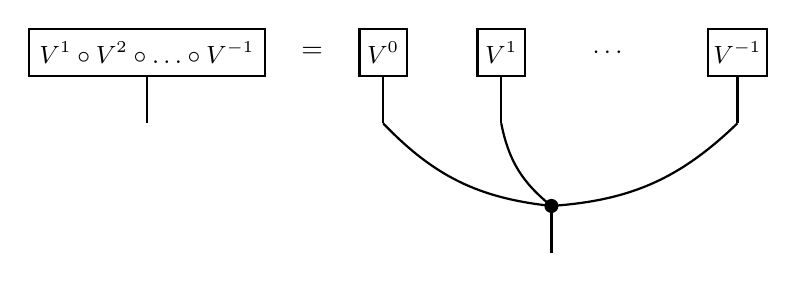
\begin{tikzpicture}[scale=0.3,thick] % , baseline = -3.5pt


\begin{scope}[shift={(-10,0)}]

\draw (-3,1) rectangle (7,3);
\node[anchor=center] (text) at (2,2) {\small $V^1\circ V^2 \circ \ldots \circ V^{\atomorder-1}$};
\draw (2,-1)--(2,1) node[midway,right] {\tiny $\catvariable$};

\node[anchor=center] (text) at (9,2) {${=}$};

\end{scope}



\draw (1,1) rectangle (3,3);
\node[anchor=center] (text) at (2,2) {\small $V^0$};
\draw (2,-1)--(2,1) node[midway,right] {\tiny $\catvariable$};


\begin{scope}[shift={(5,0)}]

\draw (1,1) rectangle (3,3);
\node[anchor=center] (text) at (2,2) {\small $V^1$};
\draw (2,-1)--(2,1) node[midway,right] {\tiny $\catvariable$};

\end{scope}

\node[anchor=center] (text) at (11.5,2) {\small $\cdots$};


\begin{scope}[shift={(15,0)}]

\draw (0.75,1) rectangle (3.25,3);
\node[anchor=center] (text) at (2,2) {\small $V^{\atomorder-1}$};
\draw (2,-1)--(2,1) node[midway,right] {\tiny $\catvariable$};

\end{scope}


\draw[fill] (9.125,-4.5) circle (0.25cm);

\draw (9.125,-4.5) to[bend right=-20] (2,-1); 
\draw (9.125,-4.5) to[bend right=-20] (7,-1); 
\draw (9.125,-4.5) to[bend right=20] (17,-1); 

\draw (9.125,-4.5) -- (9.125,-6.5) node[midway,right] {\tiny $\catvariable$};;

\end{tikzpicture}
	\end{center}
		
\end{frame}



\begin{frame}{Graphical Representation of Contractions}

\textbf{Example of a contraction}:
\begin{itemize}
	\item Four categorical variables $\nodes = \{\catvariableof{0},\catvariableof{1},\catvariableof{2},\catvariableof{3}\}$ appearing as nodes and decorated by their dimensions $\catdimof{:}$.
	\item Hyperedges  $\edge_0=\{\catvariableof{0},\catvariableof{1},\catvariableof{2}\}$, $\edge_1=\{\catvariableof{1},\catvariableof{2}\}$ and $\edge_2=\{\catvariableof{2},\catvariableof{3}\}$ decorated with tensors
	\item Contraction leaving $\{\catvariableof{1},\catvariableof{3}\}$ open, by summing over the states of $\{\catvariableof{0},\catvariableof{2}\}$
\end{itemize}

\begin{center}
	\begin{tikzpicture}[scale=0.35,thick]

    \draw (-5,-1) rectangle (9,-3);
    \node[anchor=center] (text) at (2,-2) {\corelabelsize $\contractionof{\hypercoreof{\edge_0},\hypercoreof{\edge_1},\hypercoreof{\edge_2}}{\catvariableof{1},\catvariableof{3}}$};
    \draw (0,-3)--(0,-5) node[midway,left] {\colorlabelsize $\catvariableof{1}$};
    \draw (4,-3)--(4,-5) node[midway,left] {\colorlabelsize $\catvariableof{3}$};

    \node[anchor=center] (text) at (11.5,-2) {${=}$};

    \begin{scope}
        [shift={(15,0)}]

        \draw (-1,-1) rectangle (5,-3);
        \node[anchor=center] (text) at (2,-2) {\corelabelsize $\hypercoreof{\edge_0}$};
        \draw (0,-3)--(0,-4) node[midway,right] {\colorlabelsize $\catvariableof{0}$};
        \draw (-1,-4) rectangle (1,-6);
        \node[anchor=center] (text) at (0,-5) {\corelabelsize $\ones$};

        \draw (2,-3)--(2,-5) node[midway,right] {\colorlabelsize $\catvariableof{1}$};
        \draw (4,-3)--(4,-5) node[midway,right] {\colorlabelsize $\catvariableof{2}$};


        \draw (6,-1) rectangle (10,-3);
        \node[anchor=center] (text) at (8,-2) {\corelabelsize $\hypercoreof{\edge_2}$};
        \draw (7,-3)--(7,-5) node[midway,right] {\colorlabelsize $\catvariableof{2}$};
        \draw (9,-3)--(9,-5) node[midway,right] {\colorlabelsize $\catvariableof{3}$};


        \draw (1,-7) rectangle (5,-9);
        \node[anchor=center] (text) at (3,-8) {\corelabelsize $\hypercoreof{\edge_1}$};
        \draw (2,-5)--(2,-7); % node[midway,left] {\colorlabelsize $\catvariableof{1}$};
        \draw (4,-5) to[bend right=20]  (7,-6); % node[midway,left] {\colorlabelsize $\catvariableof{2}$};
        \draw (4,-7) to[bend right=-20]  (7,-6);

        \draw[fill] (2,-6) circle (\dotsize);
        \draw (2,-6) to[bend right=20] (-1,-8); % node[midway, right]{\colorlabelsize $\catvariableof{1}$};
        \node[anchor=center] (text) at (-2,-8) {\colorlabelsize $\catvariableof{1}$};

        \draw[fill] (7,-6) circle (\dotsize);
        \draw (7,-5) -- (7,-6);
        \draw (7,-6)--(7,-7) node[midway,right] {\colorlabelsize $\catvariableof{2}$};

        \draw (6,-7) rectangle (8,-9);
        \node[anchor=center] (text) at (7,-8) {\corelabelsize $\ones$};

    \end{scope}


\end{tikzpicture}
\end{center}

\end{frame}











\begin{frame}{Curse of dimensionality of factored representations}

Tensor spaces have a problem with exponential increase of dimensions as 
	\[ \mathrm{dim}\left[ 
	\bigotimes_{\node\in\nodes} \rr^{\catdimof{\node}} 
	\right] =
	\prod_{\node\in\nodes} \catdimof{\node} \, . \]


Tensor Networks can break this curse of dimensionality by storing the decorating tensors instead
\begin{align*}
	\sum_{\edge\in\edges} \mathrm{dim}\left[  \bigotimes_{\node\in\edge} \rr^{\catdimof{\node}} \right]
	= 	\sum_{\edge\in\edges}  \left(\prod_{\node\in\edge} \catdimof{\node}\right)
\end{align*}


\begin{block}{Representation strategy}
 	Store the recipe (that is the core tensors), not the result (the contracted tensor network).
\end{block}

\end{frame}



\end{document}




\begin{frame}{Singular Value Decomposition}

Decompositions of Matrices

\end{frame}




\begin{frame}{Schmidt-Mirsky Eckard-Young Theorem}

Among the rank $r$ matrices, the matrix built from the $r$ largest singular values approximates a generic matrix best.

\end{frame}


\begin{frame}{Multiple generalization of ranks to tensor networks}

\end{frame}



